\par O confinamento quântico é um  dos fenômenos mais estudados em nanotecnologia e é causado pelo confinamento espacial dos portadores de carga em uma ou mais direções por barreiras de potencial (Miller, et al. 1984). O confinamento resulta na mudança de parâmetros referentes à estrutura eletrônica de um material. O tamanho de uma partícula interfere diretamente na sua estrutura de banda e causa mudança nas propriedades do material, como será visto adiante. (Takagahara and Takeda  1992a Wise  2000 Zhao  et  al.  2004).

\par Efeitos quânticos começam a se tornar relevantes quando a dimensão dos pontos quânticos se aproxima do raio de Bohr do éxciton do material na forma bulk (aB). O tamanho do raio de Bohr do éxciton do material bulk pode ser definido\cite{confinamento1} como:

\begin{equation}
	\label{confinamento_1}
	a_{B} = \epsilon \frac{m}{m^{\ast}}a_{0},
\end{equation}
onde $\epsilon$ é a constante dielétrica do material, $m^{\ast}$ é a massa efetiva da partícula, $m$ é a massa do elétron e $a_{0}$ é o raio de Bohr do átomo de hidrogênio.
 
\par O confinamento quântico nos leva a um efeito extremamente relevante para aplicações: o colapso das bandas de energia contínuas para bandas de energia que seguem um padrão discreto e bem definido, semelhante a um átomo, ilustrado na figura X. Para que se entenda o porquê desse efeito de confinamento, vamos analisar o conceito de densidade de estados para os materiais.
%TODO - Conferir referência
\begin{figure}[H]
  \caption{Efeito de confinamento na banda de energia (Adaptado de \cite{bulk2})}
  \centering
  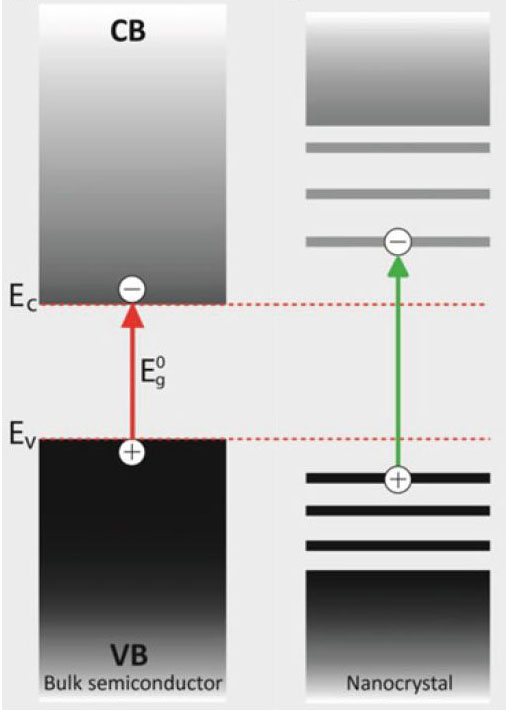
\includegraphics[width=0.5\textwidth]{images/figura9.jpg}
  \label{fig9}
\end{figure}

\subsubsection{Densidade de estado}

	\par O conceito de densidade de estados ($\rho(E)$) consiste no número de estados por volume no espaço $k$. A densidade de estados aparece em diversas áreas da Física, como, por exemplo, na termodinâmica e na óptica, na dedução da Lei de Planck para calcular densidade de estados de fótons. Em física estatística, para calcular densidades de energia nos sistemas físicos, e na mecânica quântica para calcular as probabilidades de transição envolvendo estados em um contínuo de energia, por exemplo\cite{confinamento2}.

	\par Essa densidade de estados é dada por:

	\begin{equation}
		\label{confinamento_2}
		\rho(E) = \frac{dN}{dE},
	\end{equation}
	em que $N$ é o número total de estados por espaço e $E$ é a energia do estado.

	\par A densidade de estado pode ser analisada para os casos de três, duas, uma e zero dimensões livres, como podemos ver na tabela presente na figura \ref{fig10}:

	\begin{figure}[H]
	  \caption{Classificação de estruturas confinadas}
	  \centering
	  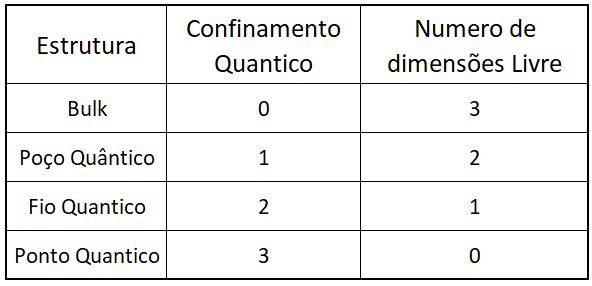
\includegraphics[width=0.65\textwidth]{images/figura10.jpg}
	  \label{fig10}
	\end{figure}

	\par Nesse tópico do trabalho será analisada a densidade de estados para os pontos quânticos, que consiste no caso de zero dimensões livres (0D). Porém, para que fique mais claro o argumento utilizado para obtenção da expressão matemática que rege a densidade de estados no caso 0D, é conveniente que se entenda como se obtém a densidade de estado para qualquer dimensão livre. Por exemplo, utilizaremos o caso mais simples, que consiste em apenas uma dimensão livre (1D), nos chamados fios quânticos.

	\begin{figure}[H]
	  \caption{Fio quântigo inserido no espaço recíproco $k$}
	  \centering
	  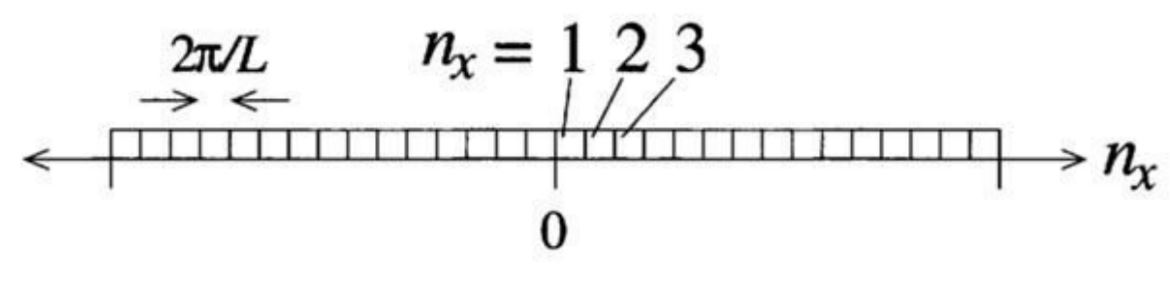
\includegraphics[width=0.8\textwidth]{images/figura11.jpg}
	  \label{fig11}
	\end{figure}

	\par O número de estados $N$ é igual ao comprimento do fio ($2k$), dividido pelo comprimento ocupado por um estado $\left(\frac{2\pi}{L}\right)$ e dividido pelo comprimento no espaço real. Tem-se\cite{confinamento3} então

	\begin{equation}
		\label{confinamento_3}
		N = 2k \cdot \frac{1}{\frac{2\pi}{L}} \cdot \frac{1}{L} \cdot 2
	\end{equation}
	onde o fator 2 surge devido à degeneração do spin.

	\par Logo, N e sua derivada:

	\begin{align}
		\label{confinamento_4}
		N^{1D} = \frac{4k}{2\pi}\\
		\frac{dN^{1D}}{dk} = \frac{2}{\pi}		
	\end{align}

	\par Portanto, definindo a densidade de estados utilizando a regra da cadeia
	\begin{equation}
		\label{confinamento_5}
		\rho^{1D}(E) = \frac{dN^{1D}}{dE} = \frac{dN^{1D}}{dk}\ \frac{dk}{dE}
	\end{equation}

	%TODO - REFERENCIAR
	\par É possível calcular o termo $\frac{dk}{dE}$ utilizando a energia do elétron livre dada na equação REFERENCIAR

	\begin{equation}
		\label{confinamento_6}
		 \frac{dk}{dE} = \left(\frac{2m^{\ast}}{\hbar^2}\right)^{\frac{1}{2}} \frac{E^{-\frac{1}{2}}}{2}
	\end{equation}

	\par Da equação \eqref{confinamento_4} e \eqref{confinamento_6}, subsititui-se em \eqref{confinamento_5}
	\begin{align}
		\label{confinamento_7}
		\rho^{1D}(E) &= \frac{2}{\pi} \left(\frac{2m^{\ast}}{\hbar^2}\right)^{\frac{1}{2}} \frac{E^{-\frac{1}{2}}}{2}\\
		\rho^{1D}(E) &= \left(\frac{2m^{\ast}}{\hbar^2}\right)^{\frac{1}{2}} \frac{1}{\pi E^{-\frac{1}{2}}},
	\end{align}
	sendo esta, a densidade de estado para 1D.

	\par De forma análoga, obtém-se os valores das desnidades de estado para todas as dimensões. A tabela expressa na figura mostra os resultados:

	\begin{figure}[H]
	  \caption{Tabela das densidades de estado para as três dimensões. Extraído de \cite{confinamento3}}
	  \centering
	  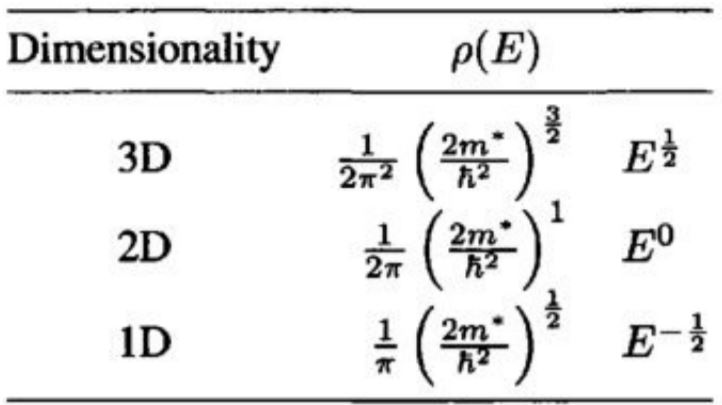
\includegraphics[width=0.6\textwidth]{images/figura12.jpg}
	  \label{fig12}
	\end{figure}

	\par No entanto a situação para os pontos quânticos é diferente. Como o elétron no ponto quântico está confinado nas 3 dimensões, não há espaço $k$ para ser preenchido e todos os estados disponíveis existem apenas em energias discretas. Portanto, pode-se descrever a densidade de estados com o \textbf{delta de Dirac}. 

	\begin{equation}
		\label{confinamento_8}
		 \rho(E)_{0D} = 2\delta(E-E_{c}),
	\end{equation}
	onde $\delta$ representa o delta de Dirac e $E_{c}$ é a energia de confinamento do elétron.

	\par A figura  apresenta gráficos indicadores de densidade de estado para todas as dimensões.

	\begin{figure}[H]
	  \caption{Gráficos da densidade de estado em todas as dimensões}
	  \centering
	  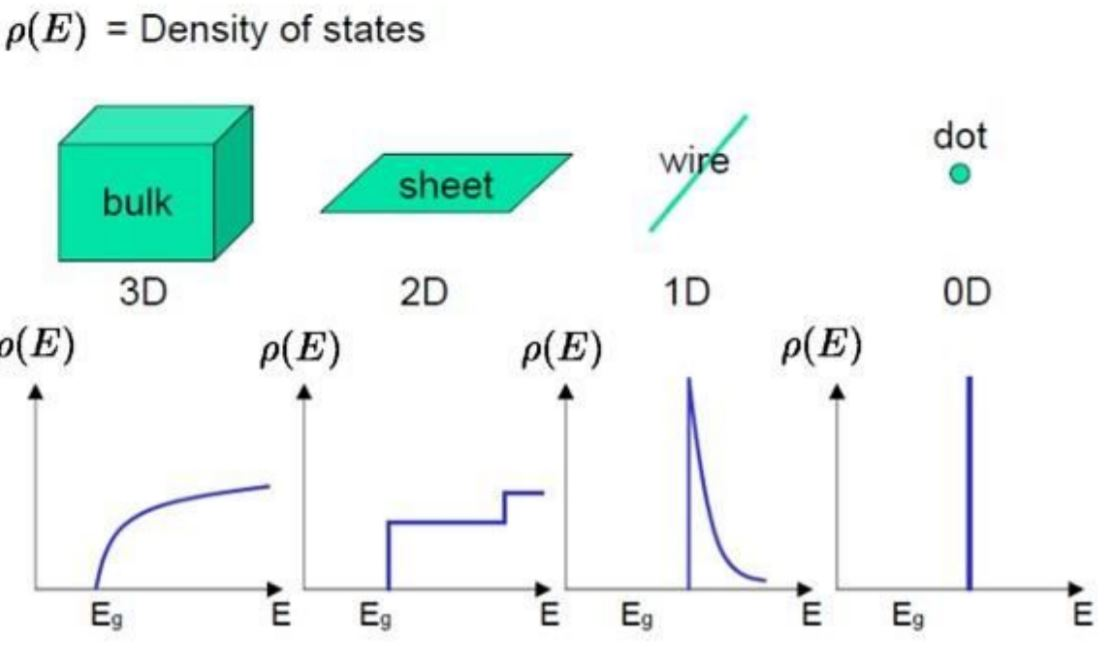
\includegraphics[width=0.6\textwidth]{images/figura13.jpg}
	  \label{fig13}
	\end{figure}

	\par Observando os resultados de densidade de estados para os pontos quânticos, comprova-se que de fato existem apenas alguns níveis de energia bem definidos e discretos nos quais o elétron pode ocupar um estado. O ponto quântico pode, por isso, ser chamado de átomo artificial. 

\subsubsection{Equação de Brus}
	
	\par Como visto anteriormente, no material bulk a estrutura eletrônica dos materiais é constituída por  bandas de energia  e, quando as dimensões do material são reduzidas, haverá uma alteração na estrutura eletrônica do material devido aos efeitos de confinamento. Seria interessante quantificar a relação entre as mudanças na estrutura eletrônica de um ponto quântico com o seu tamanho. Uma equação desse tipo seria muito importante para caracterização de QD’s dado que é possível estimar o tamanho de uma partícula a partir da medição de alguma de suas características eletrônicas, como espectro de emissão. Com esse objetivo, L.E. Brus, um premiado cientista americano, desenvolveu uma teoria que nos fornecesse tal fórmula.
 
	\par Como vimos anteriormente, quando um elétron é excitado da banda de valência para a banda de condução, ele deixa para trás uma região positiva chamada de buraco. A ligação resultante desse par elétron-buraco é o éxciton e pode ser aproximada por um modelo de partícula na caixa da mecânica quântica. Para explicar o comportamento do éxciton, o modelo de Brus será deduzido. A seguinte dedução do teorema de Brus foi baseada na dedução feita por Kippeny et al (2002).

	\par O modelo de Brus faz as seguintes aproximações: 

	\par 1 - Considera-se um nanocristal esférico e de raio R.
 
	\par 2 - As cargas e espaços ocupados que não são do éxciton são desconsiderados.
 
	\par 3 - A energia potencial fora do nanocristal é infinita, ou seja, o éxciton está sempre dentro da região delimitada pelo raio do nanocristal.
 
	\par Explora-se primeiramente o hamiltoniano de apenas uma partícula carregada (e não um éxciton) num nanocristal:

	\begin{align}
		\label{confinamento_9}
		\displaystyle \mathcal{H} &= -\frac{\hbar^2}{8\pi^2m_{c}}\nabla^2_{c} + V^{\star}\\
		\displaystyle 
			V^{\star} &=
			\left\{
	          \begin{array}{ll}
	            \displaystyle 0,\ r \leq R\\
	            \displaystyle \infty, r > R
	          \end{array}
	        \right.
	\end{align}
	onde $m_{c}$ é a massa efetiva da carga e $r$ é a distância da carga em relação ao centro do ponto quântico.
	
	\par A solução da equação de Schrodinger para esse caso pode ser obtida como no caso da partícula na caixa. Os autovalores e autovetores modificados para coordenadas esféricas são: 

	\begin{align}
		\label{confinamento_10}
	      \begin{array}{ll}
	        \displaystyle \Psi_n(r) = \frac{1}{r\sqrt{2\pi R}}\sin\left(\frac{n\pi r}{R}\right)\\
	        \displaystyle E_{n} = \frac{\hbar^2 n^2}{8m_{c}R^2},\ n=1,2,3,...
	      \end{array}
	\end{align}

	\par Percebe-se que conforme se aumenta o raio do nanocristal, as energias de absorção decrescem.
	Porém, a criação do éxciton envolve um par elétron-buraco. Para esse caso, o Hamiltoniano fica:

	\begin{equation}
		\label{confinamento_11}
		\mathcal{H} = -\frac{\hbar^2}{8\pi^2 m_{e}}\nabla^2_{e} - \frac{\hbar^2}{8\pi^2 m_{h}}\nabla^2_{h}
			+ V^{\star}(S_{e}, S_{h}),
	\end{equation}
	onde $S_{e}$ e $S_{h}$ são as posições do elétron e do buraco, respectivamente. $m_{e}$ é a massa efetiva do elétron e $m_{h}$ a massa efetiva do buraco.
	
	\par A parte potencial da equação acima pode ser dividida em duas partes: a primeira parte, para $r<R$, é a atração coulombiana entre o elétron e o buraco, da seguinte maneira:

	\begin{equation}
		\label{confinamento_12}
		V^{\star}_{Coul}(S_{e}, S_{h}) = -\frac{e^2}{4\pi\epsilon_{b}\epsilon_{0}|S_{e} - S_{h}|}
	\end{equation}
	onde $\epsilon_{b}$ é a constante dielétrica para o material bulk e $\epsilon_{0}$ é a permissividade no vácuo.

	\par O segundo termo importante desse potencial é devido ao efeito de polarização. Isso acontece devido à polarização causada no cristal por uma carga. Esse efeito afeta a energia da segunda carga. O termo de polarização é dado por:

	\begin{equation}
		\label{confinamento_13}
		V^{\star}_{pol}(S_{e}, S_{h}) = \frac{e^2}{2} \sum_{k=1}^{\infty} \alpha_{k}
			\frac{S_{e}^{2k} + S_{h}^{2k}}{R^{2k+1}}
	\end{equation}
	onde $\alpha$ é dado por:

	\begin{equation}
		\label{confinamento_14}
		\alpha_{k} = \frac{(\epsilon-1)(k+1)}{4\pi \epsilon_{b} \epsilon_{0}(\epsilon k + k + 1)}; \epsilon = \frac{\epsilon_{b}}{\epsilon_{out}}
	\end{equation}
	onde $\epsilon_{out}$ é a constante dielétrica do meio que cerca o ponto quântico.

	\par Combinando as equações \eqref{confinamento_11}, \eqref{confinamento_12}, \eqref{confinamento_13} e \eqref{confinamento_14}, o hamiltoniano total para o sistema elétron-buraco no nanocristal é:


